% 网络编程 Course Project 1 实验报告
% 编译：xelatex report.tex（运行两次以生成目录），或 latexmk -xelatex report.tex
\documentclass[a4paper,zihao=-4]{ctexart}

% ---------------- 需要填写的信息 ----------------
\newcommand{\reponame}{{\normalsize\url{https://github.com/panwhity-crypto/mcast-chat}}}
% ------------------------------------------------

\usepackage[a4paper,top=2.5cm,bottom=2.5cm,left=2.6cm,right=2.6cm]{geometry}
\usepackage{graphicx}
\usepackage{booktabs}
\usepackage{tabularx}
\usepackage{array}
\usepackage{enumitem}
\usepackage{fancyvrb}
\usepackage{xcolor}
\usepackage{caption}
\usepackage{float}
\usepackage{fancyhdr}
\usepackage{tikz}
\usetikzlibrary{arrows.meta,positioning,calc,fit}
\usepackage[hidelinks]{hyperref}

% 字体：Ubuntu 上可用 sudo apt install fonts-noto-cjk 安装
\setCJKmainfont{Noto Serif CJK SC}[BoldFont={Noto Serif CJK SC Bold}]
\setCJKsansfont{Noto Sans CJK SC}[BoldFont={Noto Sans CJK SC Bold}]
\setCJKmonofont{Noto Sans Mono CJK SC}
\setmonofont{DejaVu Sans Mono}[Scale=0.88]

\xeCJKDeclareCharClass{CJK}{"25B6}
\linespread{1.3}
\emergencystretch=3em
\setlength{\parskip}{0.3em}
\setlist{itemsep=0.2em,topsep=0.3em,leftmargin=2em}

\ctexset{
  section = {
    name = {,、},
    aftername = {},
    number = \chinese{section},
    format = \sffamily\Large\bfseries\raggedright,
    beforeskip = 1.2em, afterskip = 0.8em,
  },
  subsection = {
    number = \arabic{section}.\arabic{subsection},
    format = \sffamily\large\bfseries\raggedright,
    beforeskip = 0.9em, afterskip = 0.5em,
  },
}

\captionsetup{font=small,labelsep=quad}
\renewcommand{\arraystretch}{1.25}
\newcolumntype{Y}{>{\raggedright\arraybackslash}X}

% 代码块
\definecolor{codebg}{RGB}{246,247,249}
\definecolor{codeframe}{RGB}{210,214,220}
\DefineVerbatimEnvironment{code}{Verbatim}{fontsize=\footnotesize,frame=single,
  framesep=3mm,rulecolor=\color{codeframe},baselinestretch=1.05}
\newcommand{\inl}[1]{\texttt{#1}}

\pagestyle{fancy}
\fancyhf{}
\fancyhead[L]{\small 网络编程 Course Project 1}
\fancyhead[R]{\small 带文件传输功能的多播聊天工具}
\fancyfoot[C]{\small \thepage}
\renewcommand{\headrulewidth}{0.4pt}

\begin{document}

% ================================================================ 封面
\begin{titlepage}
  \centering
  \vspace*{3cm}
  {\sffamily\Huge\bfseries 网络编程\par}
  \vspace{0.8cm}
  {\sffamily\LARGE Course Project 1 实验报告\par}
  \vspace{2.5cm}
  {\Large\bfseries 带文件传输功能的多播聊天工具\par}
  \vspace{3cm}
  {\large
  \begin{tabular}{r@{\quad}l}
    \toprule
    题\qquad 目： & 第 3 题\ 带文件传输功能的多播聊天工具 \\
    姓\qquad 名： & 潘怀宇 \\
    实验环境： & Ubuntu 24.04，C 语言，GTK3，OpenSSL \\
    源码仓库： & \reponame \\
    完成日期： & 2026 年 11 月 18 日 \\
    \bottomrule
  \end{tabular}\par}
  \vfill
\end{titlepage}

\tableofcontents
\thispagestyle{empty}
\newpage
\setcounter{page}{1}

\noindent\textbf{实验概述：}这次大作业我选的是第 3 题“带文件传输功能的多播聊天工具”。最后在 Ubuntu 上用 C 语言完成了一个不需要服务器的多播聊天程序，界面用的是 GTK3，加密用的是 OpenSSL，题目要求的 a～d 四项都实现了，自己写的测试也全部通过。代码约 4700 行（含测试）。

% ================================================================ 一
\section{实验目的与要求}

之前做的实验基本都是 TCP 的客户端/服务器模式，这次题目明确要求用多播实现 1-N 的聊天，而且特别强调“做成聊天室的该项考核不合格”。所以我理解这次实验的重点是：不能有一个中心服务器来转发消息，每个人都要把消息直接发到多播组里，再由网络送到组里的每一台机器。

我对各项要求的理解和最后的完成情况：

\begin{enumerate}
  \item \textbf{a. 文字聊天}：直接把文字多播到组地址就行，这部分最简单。已完成。
  \item \textbf{b. 文件传输并能播放}：难点在于 UDP 不可靠，一个数据报也放不下整个文件，需要自己分片、重组，还要确认收到的文件是完整的。已完成，收到的音视频可以点击用系统播放器播放。
  \item \textbf{c. 成员管理}：要能显示当前有哪些成员，并且能删除成员。老师在这一项旁边批注了“不需要加入多播组”和“能做到但是踢不出去”，所以我重点考虑了怎么让“删除”真正有效。已完成。
  \item \textbf{d. 非对称密钥加密（加分项）}：用 RSA 分发一把共同的 AES 组密钥，再用 AES 加密聊天内容和文件。已完成。
\end{enumerate}

另外，老师说这次不要求做差错控制。我还是实现了一个简单的丢包重传，但默认是关闭的，需要加 \inl{--retransmit} 参数才会打开。

% ================================================================ 二
\section{实验环境}

\begin{table}[H]
  \centering
  \caption{实验环境}
  \begin{tabularx}{0.85\linewidth}{lY}
    \toprule
    项 & 配置 \\
    \midrule
    操作系统 & Ubuntu 24.04 LTS（20.04 / 22.04 同样适用） \\
    编译器 & gcc 13.3，C11，\inl{-Wall -Wextra} 无警告 \\
    图形界面 & GTK 3.24 \\
    加密库 & OpenSSL 3.0（libcrypto） \\
    并发 & POSIX 线程（pthread） \\
    调试与测试 & AddressSanitizer / UBSan、tcpdump、Xvfb \\
    多播参数 & 组地址 239.1.2.3，端口 50000，TTL 1 \\
    \bottomrule
  \end{tabularx}
\end{table}

我是在 Ubuntu 24.04 上开发和测试的，程序只用到了 Ubuntu 软件源里就有的库，22.04 也可以直接编译。编译和运行的步骤如下：

\begin{code}
sudo apt install build-essential pkg-config libssl-dev libgtk-3-dev
make                           # 生成 ./mcastchat
./mcastchat                    # 图形界面，启动后先填昵称
./mcastchat --cli --name 李四  # 命令行模式（没有图形界面的机器上用）
make test                      # 运行测试
\end{code}

% ================================================================ 三
\section{总体设计}

动手之前我先想清楚了一个问题：既然不能有服务器，那每个节点的地位就必须是平等的，每个人运行同一个程序，自己发自己的消息，同时接收组里所有人的消息。整体结构如图~\ref{fig:topo} 所示。

\begin{figure}[H]
  \centering
  \resizebox{\linewidth}{!}{%
\begin{tikzpicture}[
      font=\small,
      peer/.style={draw=black!45,rounded corners=4pt,minimum width=4.2cm,minimum height=1.55cm,align=center,line width=0.6pt},
      admin/.style={peer,draw=blue!70!black,fill=blue!6,line width=1pt},
      arr/.style={{Latex[length=2.2mm]}-{Latex[length=2.2mm]},draw=black!55,line width=0.7pt},
      lbl/.style={font=\footnotesize,text=black!70,align=left}]
    \node[admin] (a) at (0,0)   {\textbf{张三（管理员）}\\[1pt]聊天、发送文件\\另负责分发密钥、删除成员};
    \node[peer]  (b) at (5.2,0) {\textbf{李四（成员）}\\[1pt]聊天、发送文件\\{\color{black!60}持有当前组密钥}};
    \node[peer]  (c) at (10.4,0){\textbf{王五（成员）}\\[1pt]聊天、发送文件\\{\color{black!60}持有当前组密钥}};
    \node[draw=black!45,fill=black!4,rounded corners=4pt,minimum width=14.6cm,minimum height=1.4cm,align=center,line width=0.6pt]
      (g) at (5.2,-3.3) {\textbf{多播组 239.1.2.3:50000}\\[1pt]{\footnotesize\color{black!65}交换机按 IGMP 成员关系，把每个数据报复制给组内所有主机}};
    \draw[arr] (a.south) -- (a.south |- g.north) node[midway,right,lbl] {KEY\_DIST、KICK（签名）\\CHAT、FILE、心跳};
    \draw[arr] (b.south) -- (b.south |- g.north) node[midway,right,lbl] {CHAT、FILE、心跳};
    \draw[arr] (c.south) -- (c.south |- g.north) node[midway,right,lbl] {CHAT、FILE、心跳};
  \end{tikzpicture}}
  \caption{网络结构：所有节点直接收发多播组，没有服务器转发}
  \label{fig:topo}
\end{figure}

我认为这样的设计和“聊天室”的区别主要有三点：

\begin{itemize}
  \item 每条消息、每个文件分片都是发送者自己用 \inl{sendto()} 发到多播地址 239.1.2.3，由交换机复制给组里的每台主机；
  \item 程序里没有任何“收到别人的消息再转发出去”的代码；
  \item 后面会讲到的“管理员”也只是一个普通节点，它不转发消息，就算它下线了，其他人也能继续聊天。
\end{itemize}

\subsection{模块划分}

\begin{figure}[H]
  \centering
  \begin{tikzpicture}[
      font=\small,
      box/.style={draw=black!45,rounded corners=4pt,align=center,line width=0.6pt,minimum height=1.15cm},
      top/.style={box,minimum width=4.4cm},
      low/.style={box,minimum width=2.6cm},
      arr/.style={-{Latex[length=2mm]},draw=black!55,line width=0.7pt}]
    \node[top] (gui)   at (0,0)    {\textbf{\inl{gui.c}}\\{\footnotesize GTK3 图形界面}};
    \node[top] (cli)   at (4.9,0)  {\textbf{\inl{cli.c}}\\{\footnotesize 命令行界面}};
    \node[top] (tests) at (9.8,0)  {\textbf{\inl{tests/}}\\{\footnotesize 单元测试与多节点集成测试}};
    \node[box,draw=blue!70!black,fill=blue!6,line width=1pt,minimum width=14.2cm,minimum height=1.6cm] (node) at (4.9,-2.2)
      {\textbf{\inl{node.c} 节点协议逻辑（不依赖界面）}\\[1pt]
       {\footnotesize 成员发现与选举 · 密钥分发与换钥 · 删除成员 · 聊天收发 · 文件分片与重传}\\
       {\footnotesize\color{black!65} 接收线程 + 定时线程 + 文件工作线程，一把递归互斥锁；通过事件回调通知前端}};
    \node[low] (mem) at (-0.8,-4.4) {\textbf{\inl{members.c}}\\{\footnotesize 成员表、选举}};
    \node[low] (fx)  at (2.05,-4.4) {\textbf{\inl{filexfer.c}}\\{\footnotesize 分片重组、校验}};
    \node[low] (cr)  at (4.9,-4.4)  {\textbf{\inl{crypto.c}}\\{\footnotesize OpenSSL 加解密}};
    \node[low] (pr)  at (7.75,-4.4) {\textbf{\inl{protocol.c}}\\{\footnotesize 报文编解码}};
    \node[low] (net) at (10.6,-4.4) {\textbf{\inl{net.c}}\\{\footnotesize 多播 socket}};
    \foreach \t in {gui,cli,tests} \draw[arr] (\t.south) -- (\t.south |- node.north);
    \foreach \t in {mem,fx,cr,pr,net} \draw[arr] (\t.north |- node.south) -- (\t.north);
  \end{tikzpicture}
  \caption{单个节点的模块分层：同一个 \inl{node.c} 驱动三种前端}
  \label{fig:modules}
\end{figure}

代码上，我把协议逻辑单独放在 \inl{node.c} 里，它不依赖任何界面，只通过回调告诉界面“收到了什么”（图~\ref{fig:modules}）。这样做的好处是同一套逻辑既可以接 GTK 界面，也可以接命令行，写测试的时候还可以在一个进程里直接开好几个节点，不用每次都手动开窗口。

% ================================================================ 四
\section{详细设计与实现}

\subsection{多播 socket}

多播 socket 是整个程序的基础。我按照课上讲的多播编程步骤，在 \inl{src/net.c} 里封装了一个创建函数，每个节点只用这一个 socket 收发。关键的几行如下：

\begin{code}
/* 同一台机器上多个实例共用端口；接收缓冲区调到 4 MB */
setsockopt(fd, SOL_SOCKET, SO_REUSEADDR, &one, sizeof(one));
setsockopt(fd, SOL_SOCKET, SO_RCVBUF, &rcvbuf, sizeof(rcvbuf));
bind(fd, (struct sockaddr *)&local, sizeof(local));     /* INADDR_ANY:端口 */

/* 在指定网卡上加入多播组，内核会发出 IGMP 成员报告 */
struct ip_mreq mreq = {.imr_multiaddr = grp, .imr_interface = ifa};
setsockopt(fd, IPPROTO_IP, IP_ADD_MEMBERSHIP, &mreq, sizeof(mreq));

/* 出口网卡、TTL=1（不出本网段）、回环（同机实例互通） */
setsockopt(fd, IPPROTO_IP, IP_MULTICAST_IF, &ifa, sizeof(ifa));
setsockopt(fd, IPPROTO_IP, IP_MULTICAST_TTL, &ttl, sizeof(ttl));
setsockopt(fd, IPPROTO_IP, IP_MULTICAST_LOOP, &loop, sizeof(loop));
\end{code}

这里有几个地方需要注意：

\begin{itemize}
  \item 在同一台电脑上开几个程序互相测试时，必须设置 \inl{SO\_REUSEADDR}，否则第二个程序绑定同一端口会失败；
  \item 要打开 \inl{IP\_MULTICAST\_LOOP}，本机的其他实例才能收到；但这样自己发的包也会回到自己这里，所以接收时要按发送者 ID 把自己的包过滤掉；
  \item TTL 设为 1，只在本网段内传播；
  \item 接收缓冲区调大到 4 MB，发大文件时不容易因为缓冲区满了而丢包；
  \item 给 \inl{recvfrom} 设了 0.3 秒超时，程序退出时接收线程能及时结束。
\end{itemize}

\subsection{报文格式}

为了让各个节点能看懂彼此的消息，我自己定义了一个简单的二进制协议。每个数据报都以一个 20 字节的头部开头，格式见表~\ref{tab:header}，各类报文见表~\ref{tab:types}。

\begin{table}[H]
  \centering
  \caption{报文头部格式（网络字节序）}
  \label{tab:header}
  \begin{tabularx}{0.85\linewidth}{llY}
    \toprule
    字段 & 长度 & 说明 \\
    \midrule
    magic & 2 B & 固定 \inl{MC}，过滤无关数据包 \\
    version & 1 B & 协议版本 \\
    type & 1 B & 报文类型 \\
    sender\_id & 8 B & 节点 ID = SHA-256(RSA 公钥) 前 8 字节 \\
    seq & 4 B & 发送者自增序号 \\
    key\_epoch & 4 B & 所用组密钥版本，0 表示明文 \\
    \bottomrule
  \end{tabularx}
\end{table}

\begin{table}[H]
  \centering
  \caption{报文类型}
  \label{tab:types}
  \begin{tabularx}{\linewidth}{lYl}
    \toprule
    类型 & 载荷内容 & 保护方式 \\
    \midrule
    HELLO / HEARTBEAT & 上线时间、标志位、密钥版本、昵称、RSA 公钥 & 明文 \\
    BYE & 空 & 明文 \\
    KEY\_DIST & 目标 ID、密钥版本、RSA-OAEP(组密钥)、时间戳 & RSA 加密 + 管理员签名 \\
    KICK & 目标 ID、时间戳 & 管理员签名 \\
    CHAT & UTF-8 文本 & AES-256-GCM \\
    FILE\_META & 文件 ID、大小、分片数、SHA-256、文件名 & AES-256-GCM \\
    FILE\_CHUNK & 文件 ID、分片序号、1200 字节数据 & AES-256-GCM \\
    FILE\_END & 文件 ID、分片数 & AES-256-GCM \\
    NACK & 文件 ID、缺失分片区间 & AES-256-GCM \\
    \bottomrule
  \end{tabularx}
\end{table}

头部后面根据类型不同，放不同的内容。加密的报文我还把 20 字节头部也作为 AES-GCM 的附加认证数据，这样就算有人改了头部（比如冒充发送者），接收方解密时也会发现。此外，解析报文时每一次读取都做了边界检查，收到长度不对的包不会读越界。

\subsection{成员管理与管理员选举}

题目要求显示当前的组成员。查了资料之后我发现，IGMP 只是让路由器知道“这个网段有人要收这个组的包”，并不会告诉应用程序组里具体有谁，所以成员列表只能在应用层自己维护。我的做法是：

\begin{itemize}
  \item 程序启动后先发一个 HELLO，其他人收到后马上回一个心跳，这样新来的人很快就能看到完整的成员列表；
  \item 之后每个人每 2 秒发一次心跳，如果 6 秒都没收到某人的心跳，就认为他已经离线；
  \item 正常退出时发一个 BYE，其他人立刻把他从列表里去掉。
\end{itemize}

删除成员和分发密钥都需要有一个人来“拍板”，所以我又引入了“管理员”：

\begin{enumerate}
  \item 新节点启动后先听 2 秒，如果听到了管理员的心跳，就作为普通成员加入，等管理员发密钥；
  \item 如果没听到，说明自己是第一个来的，就自己当管理员，并生成第 1 版组密钥；
  \item 管理员退出后，剩下的人里上线最早的那个自动接任（上线时间一样就比较 ID），并换一把新密钥；
  \item 如果两个人几乎同时启动，都把自己当成了管理员，那么上线晚的那个发现对方后会自动让位。
\end{enumerate}

需要说明的是，管理员只负责发密钥和删人，聊天消息和文件还是每个人自己直接多播，管理员并不转发，所以它不是服务器。

\subsection{混合加密与密钥分发}

加分项要求用非对称密钥加密。我一开始想的是直接用 RSA 加密每条消息，但仔细想了一下行不通：RSA-2048 一次最多只能加密一百多字节，而且多播是一对多，一条消息用谁的公钥加密都不合适。所以最后采用了混合加密的方案：

\begin{enumerate}
  \item 每个节点启动时用 OpenSSL 生成自己的 RSA-2048 密钥对，公钥放在心跳里发给大家。节点 ID 就是公钥的 SHA-256 前 8 字节，收到心跳时会核对一下，防止有人冒用别人的 ID；
  \item 管理员生成一把 256 位的 AES 组密钥，分别用每个成员的公钥加密后发给他们（KEY\_DIST 报文）。由于只有对应的私钥能解开，这把密钥在网络上传输也是安全的；
  \item 之后的聊天消息和文件分片都用这把组密钥做 AES-256-GCM 加密，GCM 模式顺带还能检查数据有没有被改过；
  \item KEY\_DIST 和删人用的 KICK 报文都带上管理员的 RSA 签名，普通成员伪造的管理报文会被丢弃；
  \item 如果某个成员的 KEY\_DIST 丢了，管理员从它的心跳里能看出它的密钥版本不对，就会再发一次。
\end{enumerate}

\subsection{删除成员}

这一部分是我认为整个设计里最关键的地方。老师批注里写的“能做到但是踢不出去”，我的理解是：多播组谁都可以加入，网络层没法阻止一台主机收到组里的数据包，所以如果只是在界面上把人删掉，其实没有任何意义。

我想到的办法是“换锁”：删不掉你收包的能力，那就让你收到了也看不懂。具体步骤是：

\begin{enumerate}
  \item 管理员先多播一个带签名的 KICK 报文，告诉大家要删的是谁；
  \item 管理员生成一把新的组密钥，只用剩下成员的公钥加密后发出去，并让大家马上丢掉旧密钥；
  \item 被删的人拿不到新密钥，之后的消息和文件他虽然还能收到，但已经解不开了；
  \item 其他成员把他的 ID 加入黑名单，他发来的任何东西都不再接收；
  \item 被删的人的程序收到 KICK 后会弹出提示，并停止收发。如果他的程序被改过、不肯退出，管理员每 3 秒会再发一次 KICK。
\end{enumerate}

另外，有人正常退出时，管理员也会换一次密钥，这样离开的人也看不到以后的聊天内容。

\subsection{文件多播传输}

文件传输是在 UDP 上做的，所以分片和完整性都要自己处理。我的流程是：

\begin{enumerate}
  \item 发送方先算出整个文件的 SHA-256，把文件名、大小、分片数和哈希值放在 FILE\_META 里发出去（发两次，防止丢了）；
  \item 然后按序号一片一片地发 FILE\_CHUNK。每片数据 1200 字节，是我算过的：加上头部、加密开销和 IP/UDP 头一共 1288 字节，比以太网的 MTU 1500 小，不会被 IP 分片；
  \item 发送时限速（默认 2 MB/s），发太快的话接收方缓冲区会满；
  \item 最后发三次 FILE\_END；
  \item 接收方每收到一片，就用 \inl{pwrite} 写到文件对应的位置，并在一个位图里记下这片已经收到，重复的分片直接忽略；
  \item 全部收齐后重新算一遍 SHA-256，和 FILE\_META 里的一致才算接收成功。这时聊天框里会出现一个“▶ 播放”，点一下就用系统默认的播放器打开。
\end{enumerate}

关于丢包：因为老师说不要求差错控制，所以默认不重传，丢了分片就提示“丢失 N 个分片”。不过我还是顺手做了一个简单的补发：加上 \inl{--retransmit} 参数后，接收方发现缺片会多播一个 NACK，告诉发送方缺了哪些，发送方把几个接收方的请求合并一下再统一补发。

还有一个小细节：收到的文件名是对方发来的，如果对方故意把文件名写成 \inl{../../xxx}，就可能写到下载目录外面去。所以保存前我只取最后一段文件名，并去掉了非法字符。

\subsection{线程模型与界面}

程序里用到了多线程。每个节点有一个接收线程，专门阻塞在 \inl{recvfrom} 上收包；还有一个定时线程，每 0.25 秒负责发心跳、检查谁超时了、需不需要选新管理员、文件收齐了没有。发文件会另开一个线程，这样发大文件的时候界面不会卡住，还能继续聊天。几个线程共用的数据用一把互斥锁保护。

GTK 的界面控件只能在主线程里操作，网络线程收到消息后不能直接去改界面。我的做法是在网络线程里把事件复制一份，用 \inl{g\_idle\_add} 交给主线程，由主线程来更新聊天记录和成员列表。

% ================================================================ 五
\section{测试与结果}

网络程序光靠手点界面很难把各种情况都试到，比如丢包、管理员突然掉线、几个人同时启动等。所以我写了两类自动化测试，运行 \inl{make test} 就能全部跑一遍：

\begin{itemize}
  \item \textbf{单元测试}（\inl{tests/test\_unit.c}，61 项检查）：测报文编解码、越界读写会不会被拦住、密文被改了能不能发现、RSA 加解密和签名、恶意文件名、文件分片乱序重组等；
  \item \textbf{集成测试}（\inl{tests/test\_node.c}，48 项检查）：在一台电脑上同时开几个节点，它们之间走的是真实的 UDP 多播。丢包是在接收端按概率丢弃分片来模拟的。
\end{itemize}

最后 109 项检查全部通过。我还用 AddressSanitizer 重新编译跑了一遍（\inl{make asan}），没有发现内存越界和内存泄漏。集成测试的各个场景见表~\ref{tab:tests}。

\begin{table}[H]
  \centering
  \caption{集成测试场景与结果}
  \label{tab:tests}
  \begin{tabularx}{\linewidth}{lYc}
    \toprule
    场景 & 验证内容 & 结果 \\
    \midrule
    管理员选举与密钥分发 & 最早上线者成为管理员，三人密钥版本一致 & 通过 \\
    1-N 文本聊天 & 一人发送，其余两人都收到 & 通过 \\
    文件多播传输 & 800 KB 文件两个接收方都收到，SHA-256 一致 & 通过 \\
    删除成员 & 密钥版本 +1；被删者解不开新消息；即使拿到新密钥，它的消息也被拒收 & 通过 \\
    管理员离开 & 第二早上线者接任并分发新密钥，聊天继续 & 通过 \\
    成员超时 & 模拟崩溃后 6 秒内被移出列表 & 通过 \\
    同时启动 & 三个节点几乎同时启动，最终只有一个管理员 & 通过 \\
    明文模式 & 关闭加密时正常通信 & 通过 \\
    20\% 随机丢包 + 重传 & 600 KB 文件通过 NACK 补发后完整收到 & 通过 \\
    丢包不重传 & 丢 1 个分片，接收方报告“丢失 1 个分片” & 通过 \\
    伪造踢人报文 & 普通成员伪造的 KICK 被忽略 & 通过 \\
    普通成员删人 & 被拒绝，提示只有管理员可以删除 & 通过 \\
    \bottomrule
  \end{tabularx}
\end{table}

\subsection{抓包验证}

为了确认程序真的是在用多播、内容也确实加密了，我开了两个节点聊了几句，同时用 tcpdump 抓包（过滤条件 \inl{igmp or udp port 53400}）。从抓到的包可以看出：

\begin{itemize}
  \item 每个节点加入组的时候，内核都会发出 IGMPv3 成员报告（发往 224.0.0.22）；
  \item 所有数据报的目的地址都是 239.1.2.3，IP 头里的 TTL 是 1；
  \item 心跳包 332 字节（主要是里面带了 294 字节的公钥），KEY\_DIST 559 字节（包含 256 字节的 RSA 密文和 256 字节的签名），BYE 只有 20 字节的头部；
  \item 我发的“hello”那条消息一共 53 字节，正好是 20 字节头部 + 12 字节 nonce + 5 字节密文 + 16 字节校验标签，和设计的格式对得上，包里也看不到“hello”这几个字母。
\end{itemize}

抓包文件放在仓库的 \inl{docs/capture.pcap}，可以用 Wireshark 打开看。

\subsection{运行截图}

下面是运行截图。为了方便同时截三个人的窗口，我写了一个演示程序（\inl{make screenshots}），在一个虚拟显示器里自动打开“张三”“李四”“王五”三个窗口，依次演示聊天、发文件、删除成员和管理员交接，然后截图。

\begin{figure}[H]
  \centering
  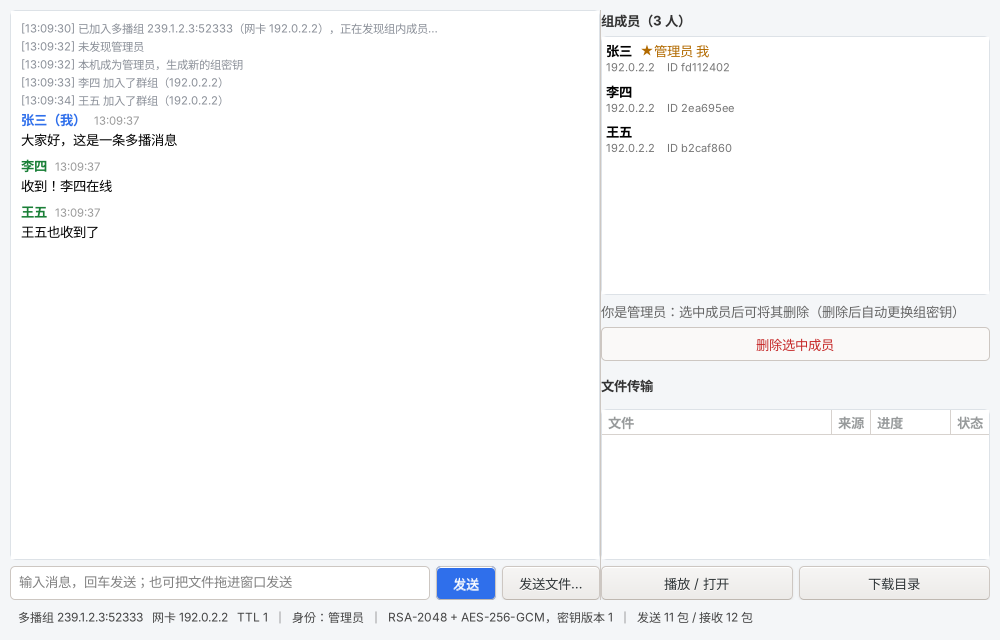
\includegraphics[width=0.92\linewidth]{figures/01_chat_admin.png}
  \caption{管理员张三的窗口：三人各发一条消息，右侧显示成员列表和管理员标记}
\end{figure}

\begin{figure}[H]
  \centering
  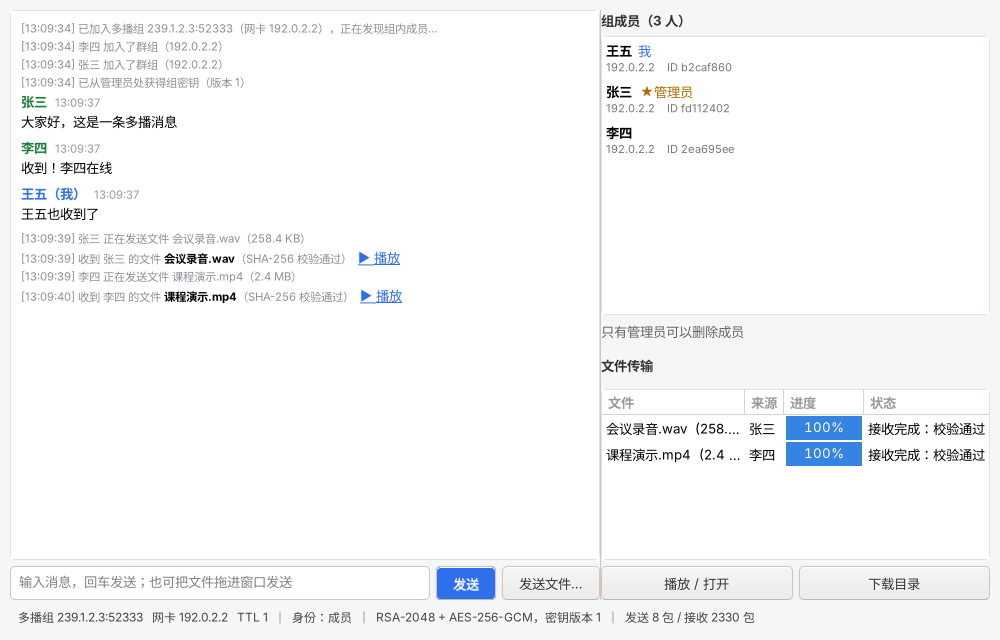
\includegraphics[width=0.92\linewidth]{figures/04_file_done.png}
  \caption{王五收到张三和李四多播的两个文件，SHA-256 校验通过，可点击“▶ 播放”}
\end{figure}

\begin{figure}[H]
  \centering
  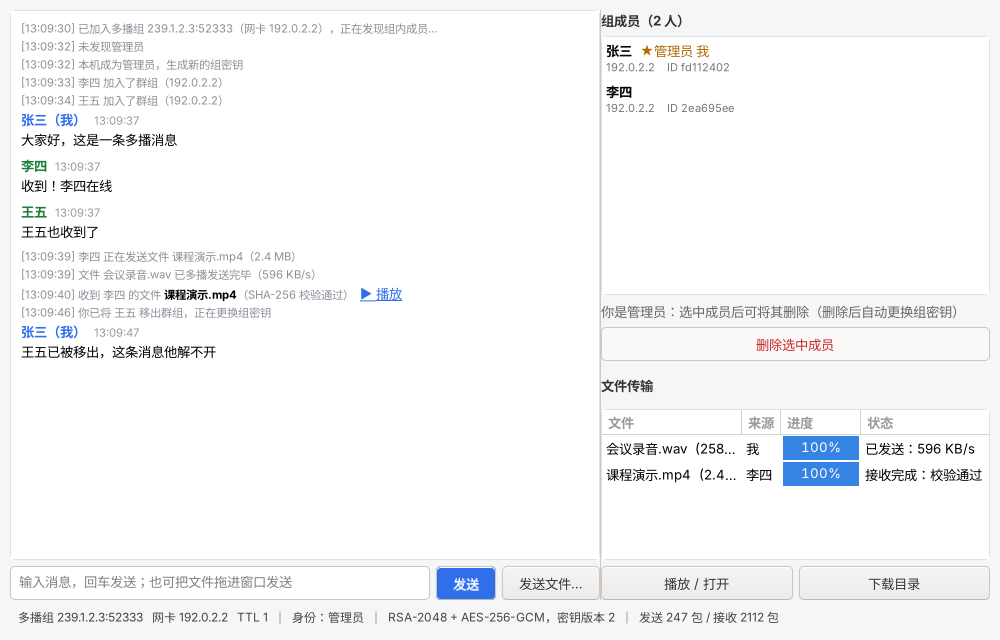
\includegraphics[width=0.92\linewidth]{figures/07_after_kick_admin.png}
  \caption{张三删除王五后：成员列表只剩两人，密钥版本变为 2}
\end{figure}

\begin{figure}[H]
  \centering
  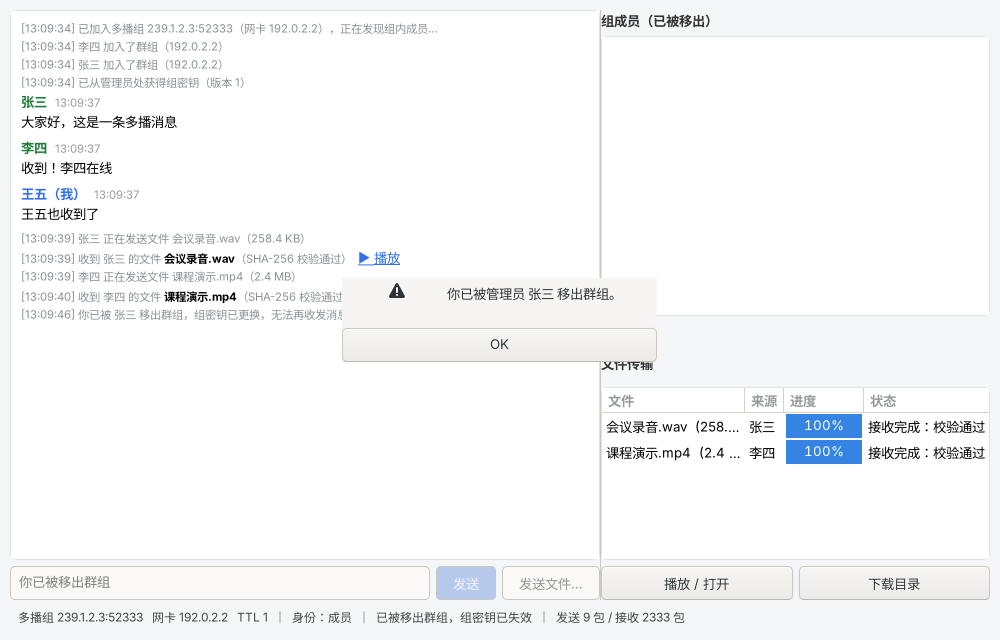
\includegraphics[width=0.92\linewidth]{figures/09_kicked.png}
  \caption{被删除的王五：收到提示，输入框禁用，状态栏显示组密钥已失效；之后张三发的消息不再出现}
\end{figure}

\begin{figure}[H]
  \centering
  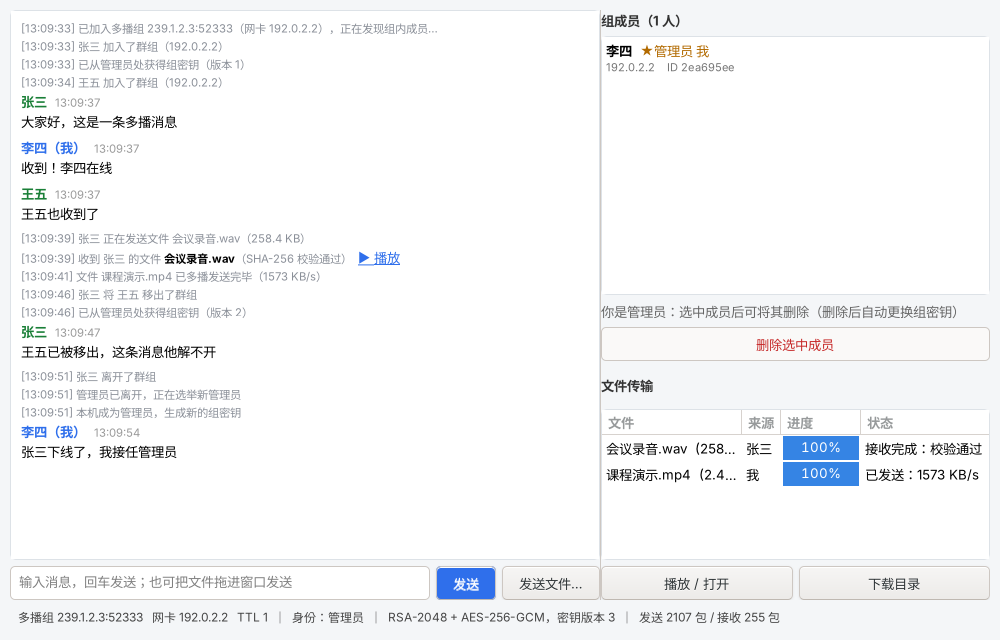
\includegraphics[width=0.92\linewidth]{figures/10_admin_handover.png}
  \caption{管理员张三下线后，李四自动接任管理员，生成第 3 版密钥}
\end{figure}

% ================================================================ 六
\section{遇到的问题与解决}

\paragraph{1. 管理员退出后又“复活”了}
测试管理员交接时发现一个奇怪的现象：管理员退出后，李四刚接任管理员，张三又出现在了成员列表里，李四还以为张三上线更早，把管理员让了回去。查了一下原因，是我退出时先发了 BYE，再去停线程，结果定时线程在 BYE 之后又发出了一个心跳。解决办法是把顺序反过来，先停掉并等待所有线程结束，再发 BYE；另外接收方对刚发过 BYE 的节点，5 秒内再收到它的心跳也直接忽略，防止网络里迟到的包造成同样的问题。

\paragraph{2. 几个人同时启动会出现两个管理员}
如果两个人几乎同时打开程序，他们在 2 秒的等待时间里都没听到管理员，就会各自把自己当成管理员，各生成一把密钥，结果谁也解不开对方的消息。我加了一个规则：管理员如果听到另一个管理员，就比较两人的上线时间，晚的一方自动让位，丢掉自己的密钥，等对方发密钥过来。

\paragraph{3. 密钥分发报文丢包}
KEY\_DIST 也是 UDP，丢了的话新成员就一直没有密钥。我的办法是让心跳里带上“我现在持有的密钥版本”，管理员发现和自己的不一致就再发一次，最多 1 秒一次。这样不用专门做确认机制，也能保证最终每个人都拿到密钥。

\paragraph{4. 发大文件容易丢包}
UDP 没有流量控制，发送方如果一口气全发出去，接收方的缓冲区很快就满了。我给发送加了限速，接收缓冲区调到 4 MB，并把分片控制在 MTU 以内，避免一个 IP 分片丢了导致整包作废。

\paragraph{5. GTK 不能在其他线程里更新界面}
GTK 不是线程安全的，接收线程收到消息后直接往聊天框里写会出问题。后来改成接收线程只复制一份事件，用 \inl{g\_idle\_add} 交给主线程去处理。

\paragraph{6. 内存检查报了一个错}
用 AddressSanitizer 和 UBSan 跑测试时，UBSan 报了一个 \inl{memcpy} 传入空指针的问题。原因是 BYE 报文没有载荷，发送时 \inl{memcpy(buf, NULL, 0)}。长度是 0 实际上不会出错，但按 C 标准这是未定义行为，我加了一个长度判断。

% ================================================================ 七
\section{总结与心得}

这次大作业比我一开始想的要复杂。写之前我以为多播聊天就是把 TCP 换成 UDP、地址换成多播地址，实际做下来才发现，多播只管“把包送到组里”，组里有谁、包丢没丢、谁有权限看，全都要在应用层自己解决。这也让我更理解了 TCP 帮我们做了多少事情。

收获比较大的有三点：

\begin{enumerate}
  \item \textbf{对多播的理解更具体了}。以前只知道概念，这次亲手设置了 \inl{IP\_ADD\_MEMBERSHIP}、TTL、回环这些选项，又用 tcpdump 看到了 IGMP 报文，对多播的工作过程有了直观的认识。
  \item \textbf{密码学可以解决网络层解决不了的问题}。“踢人”这个需求在网络层确实做不到，但换个思路，用换密钥控制“谁能看懂”，就把问题解决了。这也是我认为这次设计里最有意思的地方。
  \item \textbf{要重视测试}。管理员“复活”这种问题只在特定顺序下才出现，靠手点很难发现。把协议逻辑和界面分开、写成自动化测试之后，每次改完代码跑一遍就知道有没有改坏东西。
\end{enumerate}

另外说明一下，我一开始先用 Python 写了一版原型来验证思路，确认协议设计可行后，再按课程要求用 C 语言在 Ubuntu 上重新实现。用 C 写的时候要自己处理内存和缓冲区边界，所以我封装了带边界检查的读写函数，也用 AddressSanitizer 检查了内存问题。

程序目前还有一些不足：

\begin{itemize}
  \item 没有证书体系，成员的公钥是“第一次见到就信任”，防不了中间人攻击；而且有人谎报自己的上线时间，就能抢到管理员；
  \item 被删除的人重新生成一对 RSA 密钥，就能以新身份重新加入，需要管理员再删一次。以后可以改成新成员要管理员同意才能加入；
  \item 发 KICK 和新密钥到达之间有一个很短的空档，这期间别人用旧密钥发的消息，被删的人理论上还能解开；
  \item 不开重传时文件不保证能完整收到，只是会明确提示失败；
  \item 校园网和一些 WiFi 路由器会拦截多播，虚拟机也要用桥接模式，多台电脑演示时最好用有线交换机或者手机热点。
\end{itemize}

\end{document}
